\scanpage{49}
\margin{15}
topologiques paracompacts, à un théorème d'isomorphisme pour les \deleted{préfa} préfaisceaux [T.F Chap. II, § 5, Th. 10.2] comme on s'en convaint facilement en examinant le cas des préfaisceaux constants.

Cependant, la notion introduite ici coincide avec celle de [T.F.] dans le cas particulier des préfaisceau abéliens $P$ tel que $P(\varnothing)=0$, condition vérifiée par exemple par les préfaisceaux $\mathcal H^q(F)$ \deleted{\unsure{fa|qui}} qui s'introduisent dans la suite spectrale de Leray.
\margin{\begingroup
\setbox0=\hbox{\rotatebox{18}{aligner}}
\dimen0=\wd0 \advance\dimen0 by 8pt
\dimen2=\ht0 \advance\dimen2 by \dp0 \advance\dimen2 by 8pt
\leavevmode\rlap{\raisebox{\dimexpr-\dp0-4pt\relax}{%
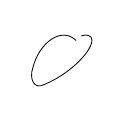
\begin{tikzpicture}[x={\dimexpr\dimen0/229\relax},y={\dimexpr-\dimen2/140\relax},line width=.3pt]
\path[use as bounding box] (0,0) rectangle (229,140);
\draw (161,26) .. controls (113,-3) and (38,30) .. (17,82) .. controls (5,103) and (20,128) .. (57,115) .. controls (130,97) and (210,53) .. (214,26) .. controls (215,16) and (194,12) .. (178,17);
\end{tikzpicture}}}%
\kern4pt\box0\kern4pt\endgroup
\figure{\begin{tikzpicture}[x=1cm,y=1cm]\draw (2.7,2.17)--(2.2,2.1);\draw (2.31,2.27)--(2.2,2.1)--(2.29,1.98);\draw (2.16,1.86)--(2.16,.34);\draw (1.92,1.52)--(2.03,1.65);\draw (2.52,0)--(2.09,.2);\draw (2.3,.27)--(2.09,.2)--(2.22,.09);\end{tikzpicture}}}

Enfin soit $\deleted{\unsure{A|\lambda}}\ a:\widehat C_A\longrightarrow\widetilde C_A$ le foncteur faisceau associé. Le foncteur $a$ est exact. Il est adjoint à gauche au foncteur $\mathcal H^0$. Le morphisme d'adjonction :
\[a\mathcal H^0\longrightarrow\operatorname{id}_{\widetilde C_A}\qquad(21)\]
est un isomorphisme (2.3.14.II).

La formule d'adjonction fournit pour tout préfaisceau d'ensembles $S$ sur $C$ et tout faisceau \begingroup
\setbox0=\hbox{d\raisebox{.65ex}{\inserted{\unsure{e|'}}}e}
\dimen0=\wd0 \advance\dimen0 by 8pt
\dimen2=\ht0 \advance\dimen2 by \dp0 \advance\dimen2 by 8pt
\leavevmode\rlap{\raisebox{\dimexpr-\dp0-4pt\relax}{%
\begin{tikzpicture}[x={\dimexpr\dimen0/73\relax},y={\dimexpr-\dimen2/54\relax},line width=.3pt]
\path[use as bounding box] (0,0) rectangle (73,54);
\draw (24,39) .. controls (33,39) and (43,36) .. (51,30);
\end{tikzpicture}}}%
\kern4pt\box0\kern4pt\endgroup $A$-modules $F$ un isomorphisme :
\margin{$\unsure{\rho}$ \raisebox{-.7ex}{\begin{tikzpicture}[x=.06cm,y=-.06cm]\draw[line width=.7pt] (0,0)--(1,.5);\end{tikzpicture}}}
\inserted{$F(aS)\xrightarrow{\sim}\mathcal H^0(F)(\unsure{S|s})$ i.e.:}
\margin{$\unsure{\rho}$}
\[
\deleted{H^0(C/aS,F)\ \unsure{\longrightarrow}\ H^0(\unsure{\widehat C|C}/S,F)\unsure{=|-}H^0(\widehat C/S,}
\]
\[H^0(\widetilde C/aS,F)\xrightarrow{\sim}H^0(\widehat C/S,\mathcal H^0(F))\qquad(22)\]

De plus si $G$ est un préfaisceau de $A$-modules tel que le faisceau associé soit nul, on a ((2.3.12.II) et (2.3.14.II)) :
\[\check{\mathcal H}^{0}(G)=0\qquad(23)\]
\margin{\begingroup
\setbox0=\hbox{\shortstack[l]{Laisser ici\\un interligne}\hspace{2.5cm}}
\dimen0=\wd0 \advance\dimen0 by 8pt
\dimen2=\ht0 \advance\dimen2 by \dp0 \advance\dimen2 by 8pt
\leavevmode\rlap{\raisebox{\dimexpr-\dp0-4pt\relax}{%
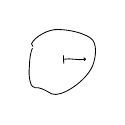
\begin{tikzpicture}[x={\dimexpr\dimen0/575\relax},y={\dimexpr-\dimen2/260\relax},line width=.3pt]
\path[use as bounding box] (0,0) rectangle (575,260);
\draw (44,71)--(32,61) .. controls (56,35) and (175,4) .. (257,7) .. controls (385,8) and (544,30) .. (556,58) .. controls (583,90) and (553,142) .. (522,161) .. controls (456,210) and (277,264) .. (201,250) .. controls (142,235) and (99,224) .. (64,227) .. controls (43,224) and (32,220) .. (29,215) .. controls (8,193) and (10,161) .. (15,144) .. controls (16,112) and (27,89) .. (40,77);

\draw (299,105)--(301,136);
\draw (306,119) .. controls (361,114) and (420,125) .. (483,119);
\draw (468,113)--(483,119)--(471,125);
\end{tikzpicture}}}%
\kern4pt\box0\kern4pt\endgroup}

Nous allons maintenant én\deleted{n}oncer les propositions liant la cohomologie de \leavevmode\rlap{\raisebox{.85ex}{\inserted{\v{\phantom{C}}}}}Cech à la cohomologie des faisceaux.

\uline{Proposition 2.2} : Le foncteur $\mathcal H^0$ transforme les faisceaux injectifs en préfaisceaux injectifs. Soit $F$ un faisceau de $A$-modules. Les faisceaux associés aux préfaisceaux $\mathcal H^q(F)$ $(q>0)$ sont nuls.
\margin{\figure{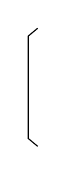
\begin{tikzpicture}\draw (.12,1.5)--(0,1.4)--(0,.1)--(.12,0);\end{tikzpicture}}}

\uline{Preuve} : Le foncteur faisceau associé, adjoint à gauche du foncteur $\mathcal H^0$ est exact; d'où la première assertion (0.2). Le foncteur $a\mathcal H^0$ est isomorphe au foncteur identique (formule (21)) d'où la deuxième assertion.

\uline{Proposition 2.3} : Soit $S$ un préfaisceau d'ensembles sur $C$.

Il existe une suite spectrale fonctoriel\raisebox{.45ex}{\inserted{le}} en $S$ et $F$ :
\[\deleted{H^{p+q}(C/\unsure{X|Y},F)\qquad\unsure{H}}\]
\[\vcenter{\hbox{\begingroup
\setbox0=\hbox{$\displaystyle H^{p+q}(\widetilde C/aS,F)\Longleftarrow H^p(\widehat C/S,\mathcal H^q(\unsure{\deleted{E}F|\deleted{F}E}))$}
\dimen0=\wd0 \advance\dimen0 by 18pt
\dimen2=\ht0 \advance\dimen2 by \dp0 \advance\dimen2 by 16pt
\rlap{\raisebox{\dimexpr-\dp0-8pt\relax}{%
\begin{tikzpicture}[x={\dimexpr\dimen0/647\relax},y={\dimexpr-\dimen2/74\relax},line width=.3pt]
\path[use as bounding box] (0,0) rectangle (647,74);
\draw (400,-18)..controls (401,-7) and (402,5)..(403,14);\draw (403,17)--(403,24);\draw (403,27)--(403,31);
\end{tikzpicture}}}%
\kern9pt\box0\kern9pt\endgroup}}\]
\margin{\figure{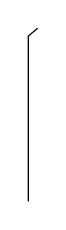
\begin{tikzpicture}\draw (.12,2.2)--(0,2.1)--(0,0);\end{tikzpicture}}}
\margin{48}
